

\tikzset{every picture/.style={line width=0.75pt}} %set default line width to 0.75pt        

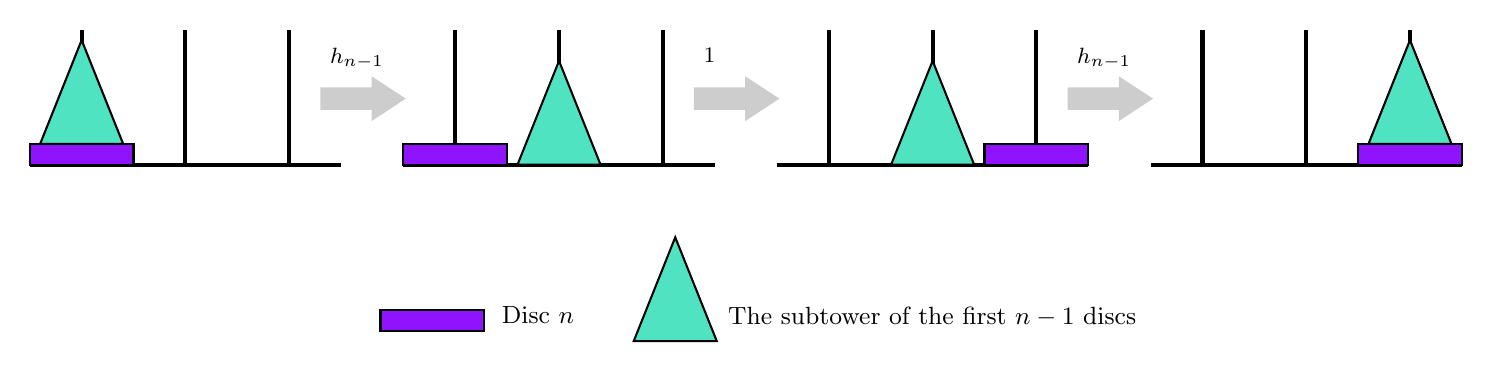
\begin{tikzpicture}[x=0.75pt,y=0.75pt,yscale=-1,xscale=1]
%uncomment if require: \path (0,241); %set diagram left start at 0, and has height of 241

%Straight Lines [id:da9282475701834738] 
\draw [line width=1.5]    (75,65) -- (75,0) ;
%Straight Lines [id:da8456727175187826] 
\draw [line width=1.5]    (125,65) -- (125,0) ;
%Straight Lines [id:da8245798231947901] 
\draw [line width=1.5]    (25,65) -- (25,0) ;
%Straight Lines [id:da31175258972263786] 
\draw [line width=1.5]    (0,65) -- (150,65) ;
%Shape: Rectangle [id:dp32704689003974163] 
\draw  [fill={rgb, 255:red, 144; green, 19; blue, 254 }  ,fill opacity=1 ] (0,55) -- (50,55) -- (50,65) -- (0,65) -- cycle ;
%Shape: Triangle [id:dp06889765992146213] 
\draw  [fill={rgb, 255:red, 80; green, 227; blue, 194 }  ,fill opacity=1 ] (25,5) -- (45,55) -- (5,55) -- cycle ;
%Straight Lines [id:da37562503022998284] 
\draw [line width=1.5]    (255,65) -- (255,0) ;
%Straight Lines [id:da46300649971101726] 
\draw [line width=1.5]    (305,65) -- (305,0) ;
%Straight Lines [id:da8693666197971948] 
\draw [line width=1.5]    (205,65) -- (205,0) ;
%Straight Lines [id:da3644645164104663] 
\draw [line width=1.5]    (180,65) -- (330,65) ;
%Shape: Rectangle [id:dp9483158274047903] 
\draw  [fill={rgb, 255:red, 144; green, 19; blue, 254 }  ,fill opacity=1 ] (180,55) -- (230,55) -- (230,65) -- (180,65) -- cycle ;
%Straight Lines [id:da21979758373938862] 
\draw [line width=1.5]    (435,65) -- (435,0) ;
%Straight Lines [id:da578932599170173] 
\draw [line width=1.5]    (485,65) -- (485,0) ;
%Straight Lines [id:da7050999519150514] 
\draw [line width=1.5]    (385,65) -- (385,0) ;
%Straight Lines [id:da4405911343620206] 
\draw [line width=1.5]    (360,65) -- (510,65) ;
%Shape: Rectangle [id:dp7574189708752779] 
\draw  [fill={rgb, 255:red, 144; green, 19; blue, 254 }  ,fill opacity=1 ] (460,55) -- (510,55) -- (510,65) -- (460,65) -- cycle ;
%Straight Lines [id:da47247880526508323] 
\draw [line width=1.5]    (615,65) -- (615,0) ;
%Straight Lines [id:da410691479483257] 
\draw [line width=1.5]    (665,65) -- (665,0) ;
%Straight Lines [id:da6499207875284638] 
\draw [line width=1.5]    (565,65) -- (565,0) ;
%Straight Lines [id:da18738816712523865] 
\draw [line width=1.5]    (540,65) -- (690,65) ;
%Shape: Rectangle [id:dp9401440468463176] 
\draw  [fill={rgb, 255:red, 144; green, 19; blue, 254 }  ,fill opacity=1 ] (640,55) -- (690,55) -- (690,65) -- (640,65) -- cycle ;
%Right Arrow [id:dp534613609568585] 
\draw  [draw opacity=0][fill={rgb, 255:red, 155; green, 155; blue, 155 }  ,fill opacity=0.5 ] (140,27.81) -- (164.71,27.81) -- (164.71,22.41) -- (181.18,33.2) -- (164.71,44) -- (164.71,38.6) -- (140,38.6) -- cycle ;
%Right Arrow [id:dp8712046365867925] 
\draw  [draw opacity=0][fill={rgb, 255:red, 155; green, 155; blue, 155 }  ,fill opacity=0.5 ] (320,27.81) -- (344.71,27.81) -- (344.71,22.41) -- (361.18,33.2) -- (344.71,44) -- (344.71,38.6) -- (320,38.6) -- cycle ;
%Right Arrow [id:dp1610359027602104] 
\draw  [draw opacity=0][fill={rgb, 255:red, 155; green, 155; blue, 155 }  ,fill opacity=0.5 ] (500,27.81) -- (524.71,27.81) -- (524.71,22.41) -- (541.18,33.2) -- (524.71,44) -- (524.71,38.6) -- (500,38.6) -- cycle ;
%Shape: Rectangle [id:dp8645342569013641] 
\draw  [fill={rgb, 255:red, 144; green, 19; blue, 254 }  ,fill opacity=1 ] (169,135) -- (219,135) -- (219,145) -- (169,145) -- cycle ;

%Shape: Triangle [id:dp547271885867356] 
\draw  [fill={rgb, 255:red, 80; green, 227; blue, 194 }  ,fill opacity=1 ] (311,100) -- (331,150) -- (291,150) -- cycle ;
%Shape: Triangle [id:dp6848694482352105] 
\draw  [fill={rgb, 255:red, 80; green, 227; blue, 194 }  ,fill opacity=1 ] (255,15) -- (275,65) -- (235,65) -- cycle ;
%Shape: Triangle [id:dp05180516619833431] 
\draw  [fill={rgb, 255:red, 80; green, 227; blue, 194 }  ,fill opacity=1 ] (435,15) -- (455,65) -- (415,65) -- cycle ;
%Shape: Triangle [id:dp8992062198078927] 
\draw  [fill={rgb, 255:red, 80; green, 227; blue, 194 }  ,fill opacity=1 ] (665,5) -- (685,55) -- (645,55) -- cycle ;

% Text Node
\draw (143.18,7.4) node [anchor=north west][inner sep=0.75pt]  [font=\footnotesize]  {$h_{n-1}$};
% Text Node
\draw (323.18,7.4) node [anchor=north west][inner sep=0.75pt]  [font=\footnotesize]  {$1$};
% Text Node
\draw (503.18,7.4) node [anchor=north west][inner sep=0.75pt]  [font=\footnotesize]  {$h_{n-1}$};
% Text Node
\draw (226,132) node [anchor=north west][inner sep=0.75pt]  [font=\small] [align=left] {Disc $\displaystyle n$};
% Text Node
\draw (335,132) node [anchor=north west][inner sep=0.75pt]  [font=\small] [align=left] {The subtower of the first $\displaystyle n-1$ discs};


\end{tikzpicture}